\documentclass{article}
\usepackage[utf8]{inputenc}
\usepackage{hyperref}
\usepackage{graphicx}

\title{NLP Project Proposal}
\author{Andreas Kuster, Viswa Virinchi, Jakub Filipek}
\date{\today}

\begin{document}

\maketitle

\section*{Citation}

Title: ner and pos when nothing is capitalized \\

\noindent
Url: \href{https://www.aclweb.org/anthology/D19-1650/}{www.aclweb.org/anthology/D19-1650/} \\

\noindent
Authors: Stephen Mayhew, Tatiana Tsygankova, Dan Roth \\

\noindent
Abstract:  \\
For those languages which use it, capitalization is an important signal for the fundamental NLP tasks of Named Entity Recognition (NER) and Part of Speech (POS) tagging. In fact, it is such a strong signal that model performance on these tasks drops sharply in common lowercased scenarios, such as noisy web text or machine translation outputs. In this work, we perform a systematic analysis of solutions to this problem, modifying only the casing of the train or test data using lowercasing and truecasing methods. While prior work and first impressions might suggest training a caseless model, or using a truecaser at test time, we show that the most effective strategy is a concatenation of cased and lowercased training data, producing a single model with high performance on both cased and uncased text. As shown in our experiments, this result holds across tasks and input representations. Finally, we show that our proposed solution gives an 8\% F1 improvement in mention detection on noisy out-of-domain Twitter data.


\section{Contributions}

\subsection*{Exercise 1a}
Task: A clear list of the scientific hypotheses evaluated in the original paper. Some papers don't make this super clear, so it can take a couple readings of the paper to understand.
\\
\\
The authors hypothesised that re-training standard NER and POS architectures with mixed cased and uncased training data would remove the dependence on casing and improves the F-score of such classification tasks. They perform experiments on cased and uncased test sets, retraining the NER and POS models using different embedding by 
\begin{itemize}
    \item Training on cased data
    \item Training on uncased data
    \item Training on concatenation of cased and uncased
    \item Training on concatenation of cased and uncased but randomly lowercasing 50\% of the data
    \item Training on cased and truecase the test data
    \item Truecase both the training and test data
\end{itemize}

They perform the same experiments with The Broad Twitter data, an informal corpus, retraining the NER model and verify their hypothesis that re-training on a mixture of cased and uncased datasets will improve F-scores




\section{Access to data}
Task: Give a short description of whether and how you can access the data used in the paper.
\\
\\
The paper describes different evaluations performed using several models and data sources. We will go through them, list all data sources, and give a summary at the end, where we describe how we can get hold of this data.


\subsection*{Evaluation 1}
Performance evaluation of modern models trained on cased text, evaluated on lowercased text.
\\
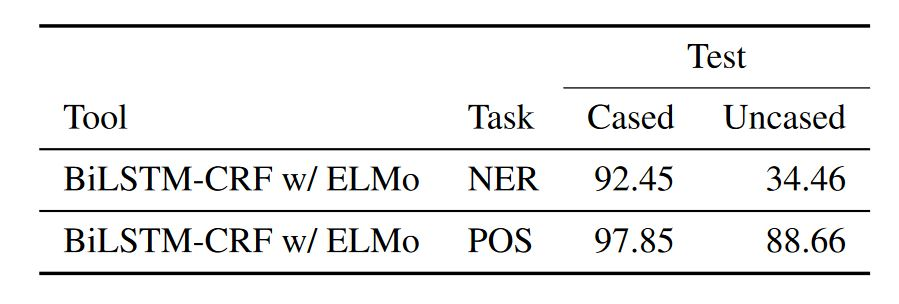
\includegraphics[width=0.5\textwidth]{stat1}
\\
Data sources:
\begin{itemize}
	\item \href{https://dl.acm.org/doi/10.3115/1119176.1119195}{CoNLL 2003}
	\item \href{https://www.seas.upenn.edu/~pdtb/}{Penn TreeBank}
\end{itemize}


\subsection*{Evaluation 2}
Truecaser performance evaluation.
\\
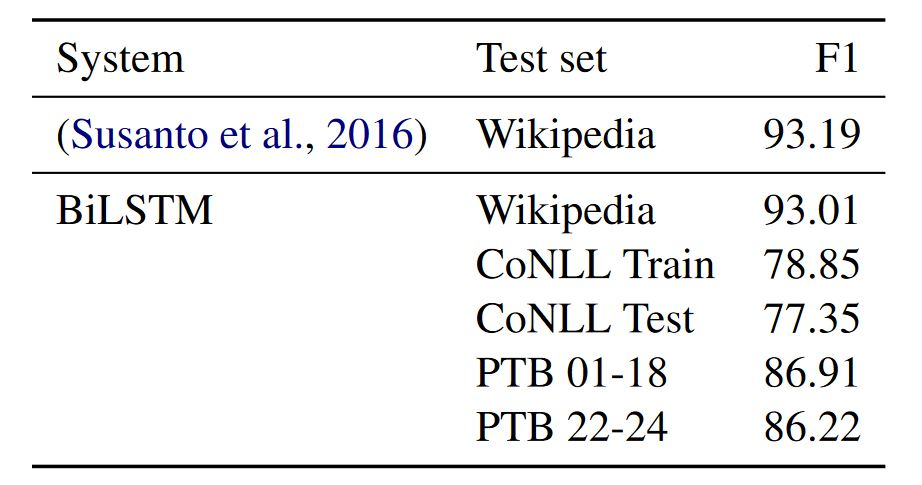
\includegraphics[width=0.5\textwidth]{stat2}
\\
Data sources:
\begin{itemize}
	\item \href{https://cs.pomona.edu/~dkauchak/simplification/}{Simplified Wikipedia}
	\item \href{https://dl.acm.org/doi/10.3115/1119176.1119195}{CoNLL 2003}
	\item \href{https://www.seas.upenn.edu/~pdtb/}{Penn TreeBank}
\end{itemize}


\subsection*{Evaluation 3} 
NER+ELMo / POS+ELMo performance evaluation on CoNLL 2003 and PTB data.
\\
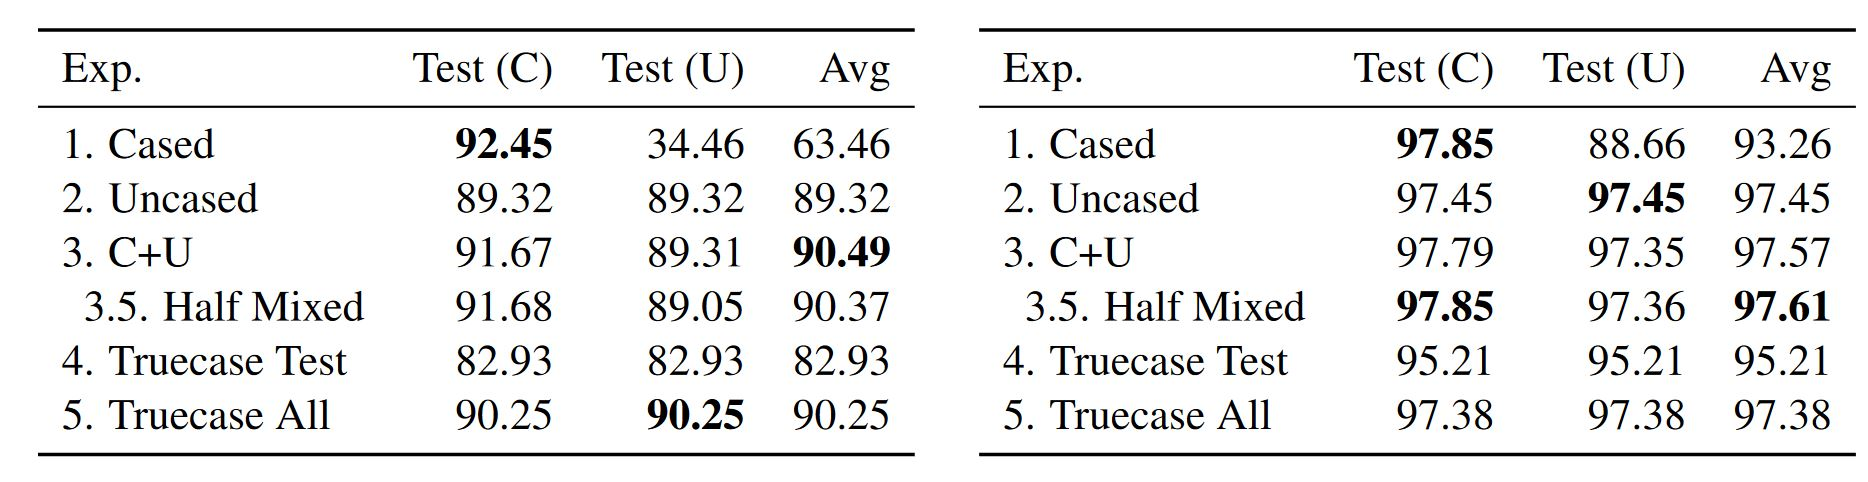
\includegraphics[width=0.5\textwidth]{stat3}
\\
Data sources:
\begin{itemize}
	\item \href{https://dl.acm.org/doi/10.3115/1119176.1119195}{CoNLL 2003}
	\item \href{https://www.seas.upenn.edu/~pdtb/}{Penn TreeBank}
\end{itemize}


\subsection*{Evaluation 4}
NER+ELMo performance evaluation on twitter data.
\\
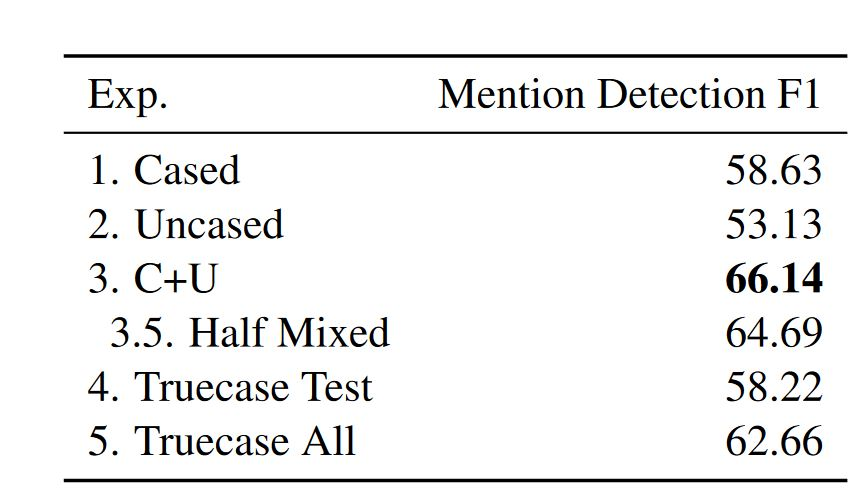
\includegraphics[width=0.5\textwidth]{stat4}
\\
Data sources:
\begin{itemize}
	\item \href{https://github.com/GateNLP/broad_twitter_corpus}{Twitter}
\end{itemize}


\subsection*{Conclusion}
The data sources are: \href{https://dl.acm.org/doi/10.3115/1119176.1119195}{CoNLL 2003}, \href{https://www.seas.upenn.edu/~pdtb/}{Penn TreeBank}, \href{https://cs.pomona.edu/~dkauchak/simplification/}{Simplified Wikipedia} and \href{https://github.com/GateNLP/broad_twitter_corpus}{Twitter}.
We were able to obtain a copy of the \textit{CoNLL 2003} and \textit{Penn TreeBank} dataset internally. Furthermore, the data from \textit{Simplified Wikipedia} and \textit{Twitter} is publicly available on the web. Therefore, we conclude that we obtained access to all required data for this project.



\section{Feasibility}
The project should be feasible because majority of models are either available pre-trained or with implemented architectures as authors specify exactly which implementation they used (mostly based on \href{https://github.com/allenai/allennlp}{AllenNLP github repo}).
There will however be a few things such as \href{https://nlp.stanford.edu/pubs/glove.pdf}{Glove word vectors}, which I could not find official implementation for (\href{https://github.com/hans/glove.py}{There is this unofficial attempt} though, which would have to be checked for correctness). Hence, overall we should not be too heavy on GPU use, which is the biggest bottleneck in such project.

Considering the fact that BiLSTM models with pre-trained weights are \href{https://github.com/UKPLab/emnlp2017-bilstm-cnn-crf/blob/master/docs/Pretrained_Models.md}{less than 500mb}, they should be easily able to fit in 8GB of memory of 1080TI. Since those are the biggest models used in paper, other should not be a problem either.

Another nice thing about this project is that every data-set used is cited, and available. One thing to note is that sometimes the labels may not be available (as in Wikipedia dataset example), but due to nature of casing tasks, labels can be created automatically at virtually zero cost.

Hence overall our work will be computationally feasible because it will mostly rely on fine-tuning models which is much cheaper than training them from scratch.

The only bottleneck can occur if there will be significant discrepancies between the paper and our results, specifically when using BiLSTM-CRF and ELMO. This can result in rather computationally heavy task of training these models from scratch. However, we do have a computational time buffer, which can be used in such case.



\end{document}